%\documentclass[a4,semhelv,landscape]{seminar}
\documentclass[landscape]{slides}
%\documentclass[pdf, default, slideBW, nocolorBG]{prosper}
\usepackage[left=0.2cm,top=0.2cm,right=0.2cm,bottom=0.2cm,nohead,nofoot]{geometry}
%\def\everyslide{\sffamily}
%\usepackage{fullpage}
\usepackage{graphicx}
\usepackage[usenames]{color}
%\usepackage{color}
\usepackage{verbatim}
\usepackage{nopageno}
\usepackage{setspace}
%\usepackage{times}
% define some nice colors
\definecolor{myred}{rgb}{0.6,0,0}
\definecolor{myblue}{rgb}{0,0.2,0.4}
\definecolor{mygreen}{rgb}{0,0.5,0.0}
\definecolor{mypurple}{cmyk}{0.5,1.0,0.0,0.0}
\definecolor{myorange}{cmyk}{0.0,0.75,1.0,0.0}
%\color{myblue}

\begin{document}
%%%%%%%%%%%%%%%%%%%%%%%%%%%%%%%%%%%%%%%%%%%%%%%%%%%%%%%%%%%%%%%%%%%%
%Slide 0 - title
\begin{slide}
\begin{center}
\large{\textbf{Validation and annotation of SARS-CoV-2 sequences using VADR}}

\normalsize

Eric Nawrocki \\

\medskip

\medskip

\medskip

\medskip

\medskip

\small
\begin{tabular}{c}
%Alejandro Sch\"{a}ffer's group \\
%\\
Computational Biology Branch \\
%National Center for Biotechnology Information\\
National Center for Biotechnology Information\\
%National Institutes of Health\\
National Library of Medicine \\
\\
\end{tabular}

\vspace{0.1in}

\includegraphics[width=2.5in]{figs/ncbi-logo}

\end{center}
\end{slide}
%%%%%%%%%%%%%%%%%%%%%%%%%%%%%%%%%%%%%%%%%%%%%%%%%%%%%%%%%%%%%%%%%%%%%%
\begin{slide}
\begin{center}
\large{\textbf{GenBank indexers handle incoming sequence submissions}}
\end{center}

\center{\includegraphics[width=9in]{figs/spheres-submission-schematic-1}}

\vfill
\end{slide}
%%%%%%%%%%%%%%%%%%%%%%%%%%%%%%%%%%%%%%%%%%%%%%%%%%%%%%%%%%%%%%%%%%%%%%
\begin{slide}
\begin{center}
\includegraphics[width=10in]{figs/vadr-title-paper}

\begin{itemize}
\item general tool for reference-based annotation of viral sequences
\item used for dengue virus and norovirus submissions since 2018
\item used for SARS-CoV-2 submissions since March 2020 
\end{itemize}

\vfill
\end{center}
\end{slide}
%%%%%%%%%%%%%%%%%%%%%%%%%%%%%%%%%%%%%%%%%%%%%%%%%%%%%%%%%%%%%%%%%%%%%%
\begin{slide}
\begin{center}
\large{\textbf{VADR assists GenBank indexers}}
\large{\textbf{Each sequence \textcolor{green}{PASSes} or \textcolor{red}{FAILs}}}
\end{center}

\center{\includegraphics[width=9in]{figs/spheres-submission-schematic-2}}

\vfill
\end{slide}
%%%%%%%%%%%%%%%%%%%%%%%%%%%%%%%%%%%%%%%%%%%%%%%%%%%%%%%%%%%%%%%%%%%%%%
\begin{slide}
\begin{center}
\large{\textbf{Indexers decide fate of \textcolor{red}{FAILing} sequences}}
\end{center}

\center{\includegraphics[width=9in]{figs/spheres-submission-schematic-3}}

\vfill
\end{slide}
%%%%%%%%%%%%%%%%%%%%%%%%%%%%%%%%%%%%%%%%%%%%%%%%%%%%%%%%%%%%%%%%%%%%%%
\begin{slide}
\begin{center}
\large{\textbf{Some sequences are sent directly back to submitter with
    error reports}}
\end{center}

\center{\includegraphics[width=9in]{figs/spheres-submission-schematic-4}}

\vfill
\end{slide}
%%%%%%%%%%%%%%%%%%%%%%%%%%%%%%%%%%%%%%%%%%%%%%%%%%%%%%%%%%%%%%%%%%%%%%
\begin{slide}
\begin{center}
\large{\textbf{VADR builds a reference model of a RefSeq and its features}}
\end{center}

\includegraphics[width=10.5in]{figs/dengue-features}

\vfill
\end{slide}
%%%%%%%%%%%%%%%%%%%%%%%%%%%%%%%%%%%%%%%%%%%%%%%%%%%%%%%%%%%%%%%%%%%%%%
\begin{slide}
\begin{center}
%\textbf{\texttt{v-annotate.pl} annotates each sequence using its
\textbf{VADR validates and annotates each input sequence \\ using its 
  best-matching model}

\begin{itemize}
\item For each sequence $S$:
\small
\begin{enumerate}
\item \textbf{Classification}: compare $S$ to all models to find best matching model $M$
\item \textbf{Coverage determination}: search $M$ against $S$ to find 'hits'
\item \textbf{Alignment}: align $S$ to $M$ and map features from $M$ to $S$
\item \textbf{Protein validation}: compare predicted CDS in $S$ to proteins
  from $M$ using BLASTX
\end{enumerate}
\end{itemize}

\emph{Different types of alerts are identified and reported at each stage}

\end{center}

\vfill
\end{slide}
%%%%%%%%%%%%%%%%%%%%%%%%%%%%%%%%%%%%%%%%%%%%%%%%%%%%%%%%%%%%%%%%%%%%%%
\begin{slide}
\begin{center}

\includegraphics[width=9.5in]{figs/v-annotate-stage1-1}

\end{center}
\vfill
\end{slide}
%%%%%%%%%%%%%%%%%%%%%%%%%%%%%%%%%%%%%%%%%%%%%%%%%%%%%%%%%%%%%%%%%%%%%%
\begin{slide}
\begin{center}

\includegraphics[width=9.5in]{figs/v-annotate-stage1-2}

\end{center}
\vfill
\end{slide}
%%%%%%%%%%%%%%%%%%%%%%%%%%%%%%%%%%%%%%%%%%%%%%%%%%%%%%%%%%%%%%%%%%%%%%
\begin{slide}
\begin{center}

\includegraphics[width=9.5in]{figs/v-annotate-stage1-2}

\includegraphics[width=10.5in]{figs/ss-class-alert-list}

\end{center}
\vfill
\end{slide}
%%%%%%%%%%%%%%%%%%%%%%%%%%%%%%%%%%%%%%%%%%%%%%%%%%%%%%%%%%%%%%%%%%%%%%
\begin{slide}
\begin{center}

\includegraphics[width=10.5in]{figs/v-annotate-stage2-1}

\end{center}
\vfill
\end{slide}
%%%%%%%%%%%%%%%%%%%%%%%%%%%%%%%%%%%%%%%%%%%%%%%%%%%%%%%%%%%%%%%%%%%%%%
\begin{slide}
\begin{center}

\includegraphics[width=10.5in]{figs/v-annotate-stage2-2}
\includegraphics[width=10in]{figs/ss-coverage-alert-list}
\end{center}

\vfill
\end{slide}
%%%%%%%%%%%%%%%%%%%%%%%%%%%%%%%%%%%%%%%%%%%%%%%%%%%%%%%%%%%%%%%%%%%%%%
\begin{slide}
\begin{center}

\includegraphics[width=10.5in]{figs/v-annotate-stage3-1}
\end{center}

\vfill
\end{slide}
%%%%%%%%%%%%%%%%%%%%%%%%%%%%%%%%%%%%%%%%%%%%%%%%%%%%%%%%%%%%%%%%%%%%%%
\begin{slide}
\begin{center}

\includegraphics[width=10.5in]{figs/v-annotate-stage3-2}
\end{center}

\vfill
\end{slide}
%%%%%%%%%%%%%%%%%%%%%%%%%%%%%%%%%%%%%%%%%%%%%%%%%%%%%%%%%%%%%%%%%%%%%%
\begin{slide}
\begin{center}

\includegraphics[width=10.5in]{figs/v-annotate-stage3-3}
\end{center}

\vfill
\end{slide}
%%%%%%%%%%%%%%%%%%%%%%%%%%%%%%%%%%%%%%%%%%%%%%%%%%%%%%%%%%%%%%%%%%%%%%
\begin{slide}
\begin{center}

\includegraphics[width=10.5in]{figs/v-annotate-stage3-4}
\includegraphics[width=10.5in]{figs/ss-alignment-alert-list}

\end{center}
\vfill
\end{slide}
%%%%%%%%%%%%%%%%%%%%%%%%%%%%%%%%%%%%%%%%%%%%%%%%%%%%%%%%%%%%%%%%%%%%%%
\begin{slide}
\begin{center}

\includegraphics[width=10.5in]{figs/v-annotate-stage4-1}

\end{center}
\vfill
\end{slide}
%%%%%%%%%%%%%%%%%%%%%%%%%%%%%%%%%%%%%%%%%%%%%%%%%%%%%%%%%%%%%%%%%%%%%%
\begin{slide}
\begin{center}

\includegraphics[width=10.5in]{figs/v-annotate-stage4-2}
\includegraphics[width=10.5in]{figs/ss-protein-alert-list}

\end{center}
\vfill
\end{slide}
%%%%%%%%%%%%%%%%%%%%%%%%%%%%%%%%%%%%%%%%%%%%%%%%%%%%%%%%%%%%%%%%%%%%%%
\begin{slide}
\begin{center}
\textbf{SARS-CoV-2 sequences in GenBank: Jan 2020 to June 2020}

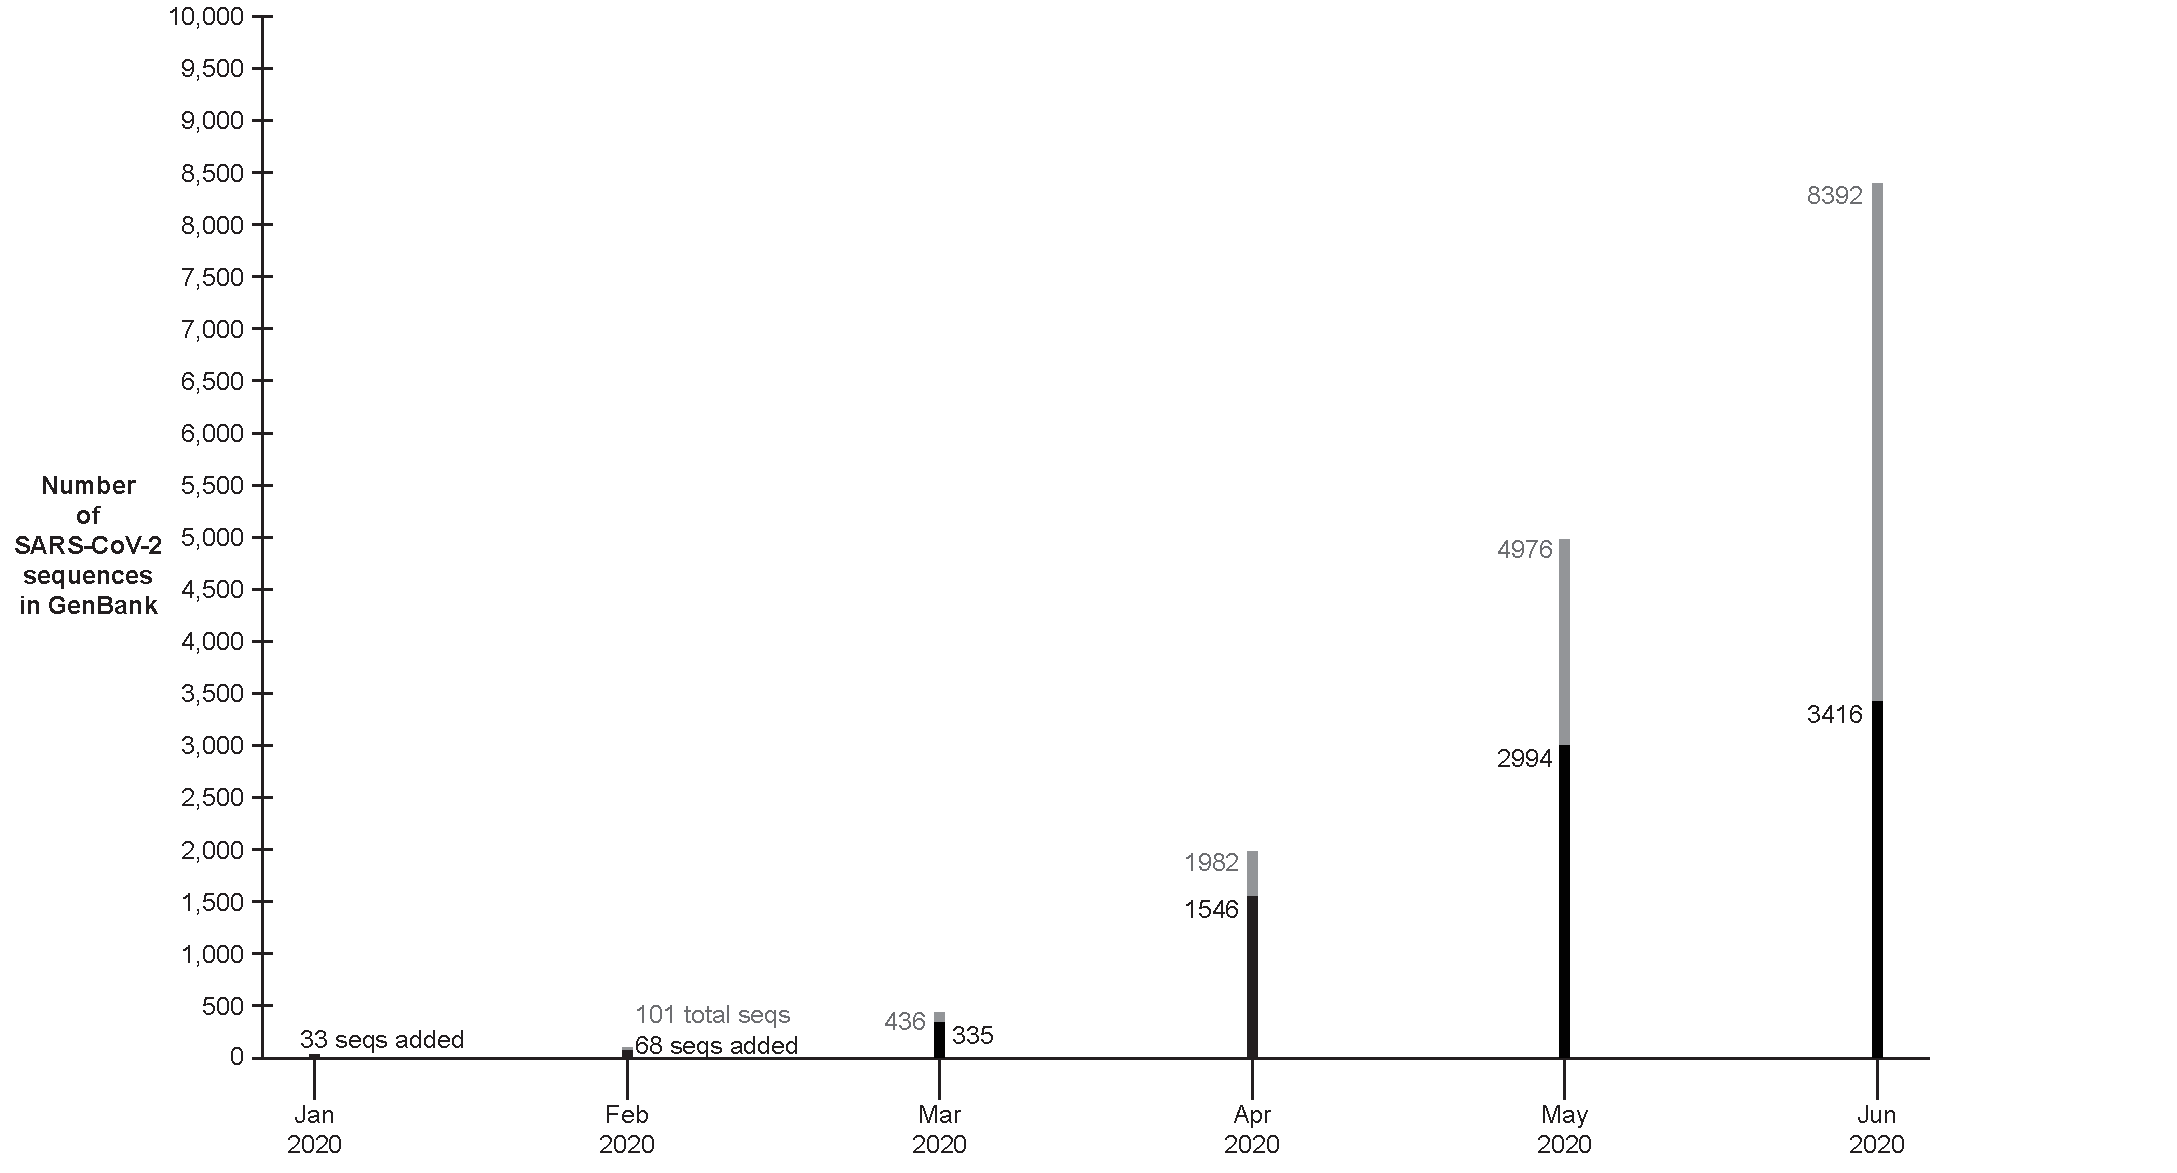
\includegraphics[width=10.5in]{figs/sars-counts-jan2020-may2020-slide1}
\end{center}

\vfill
\end{slide}
%%%%%%%%%%%%%%%%%%%%%%%%%%%%%%%%%%%%%%%%%%%%%%%%%%%%%%%%%%%%%%%%%%%%%%
\begin{slide}
\begin{center}
\textbf{VADR 1.0: functional but slow}

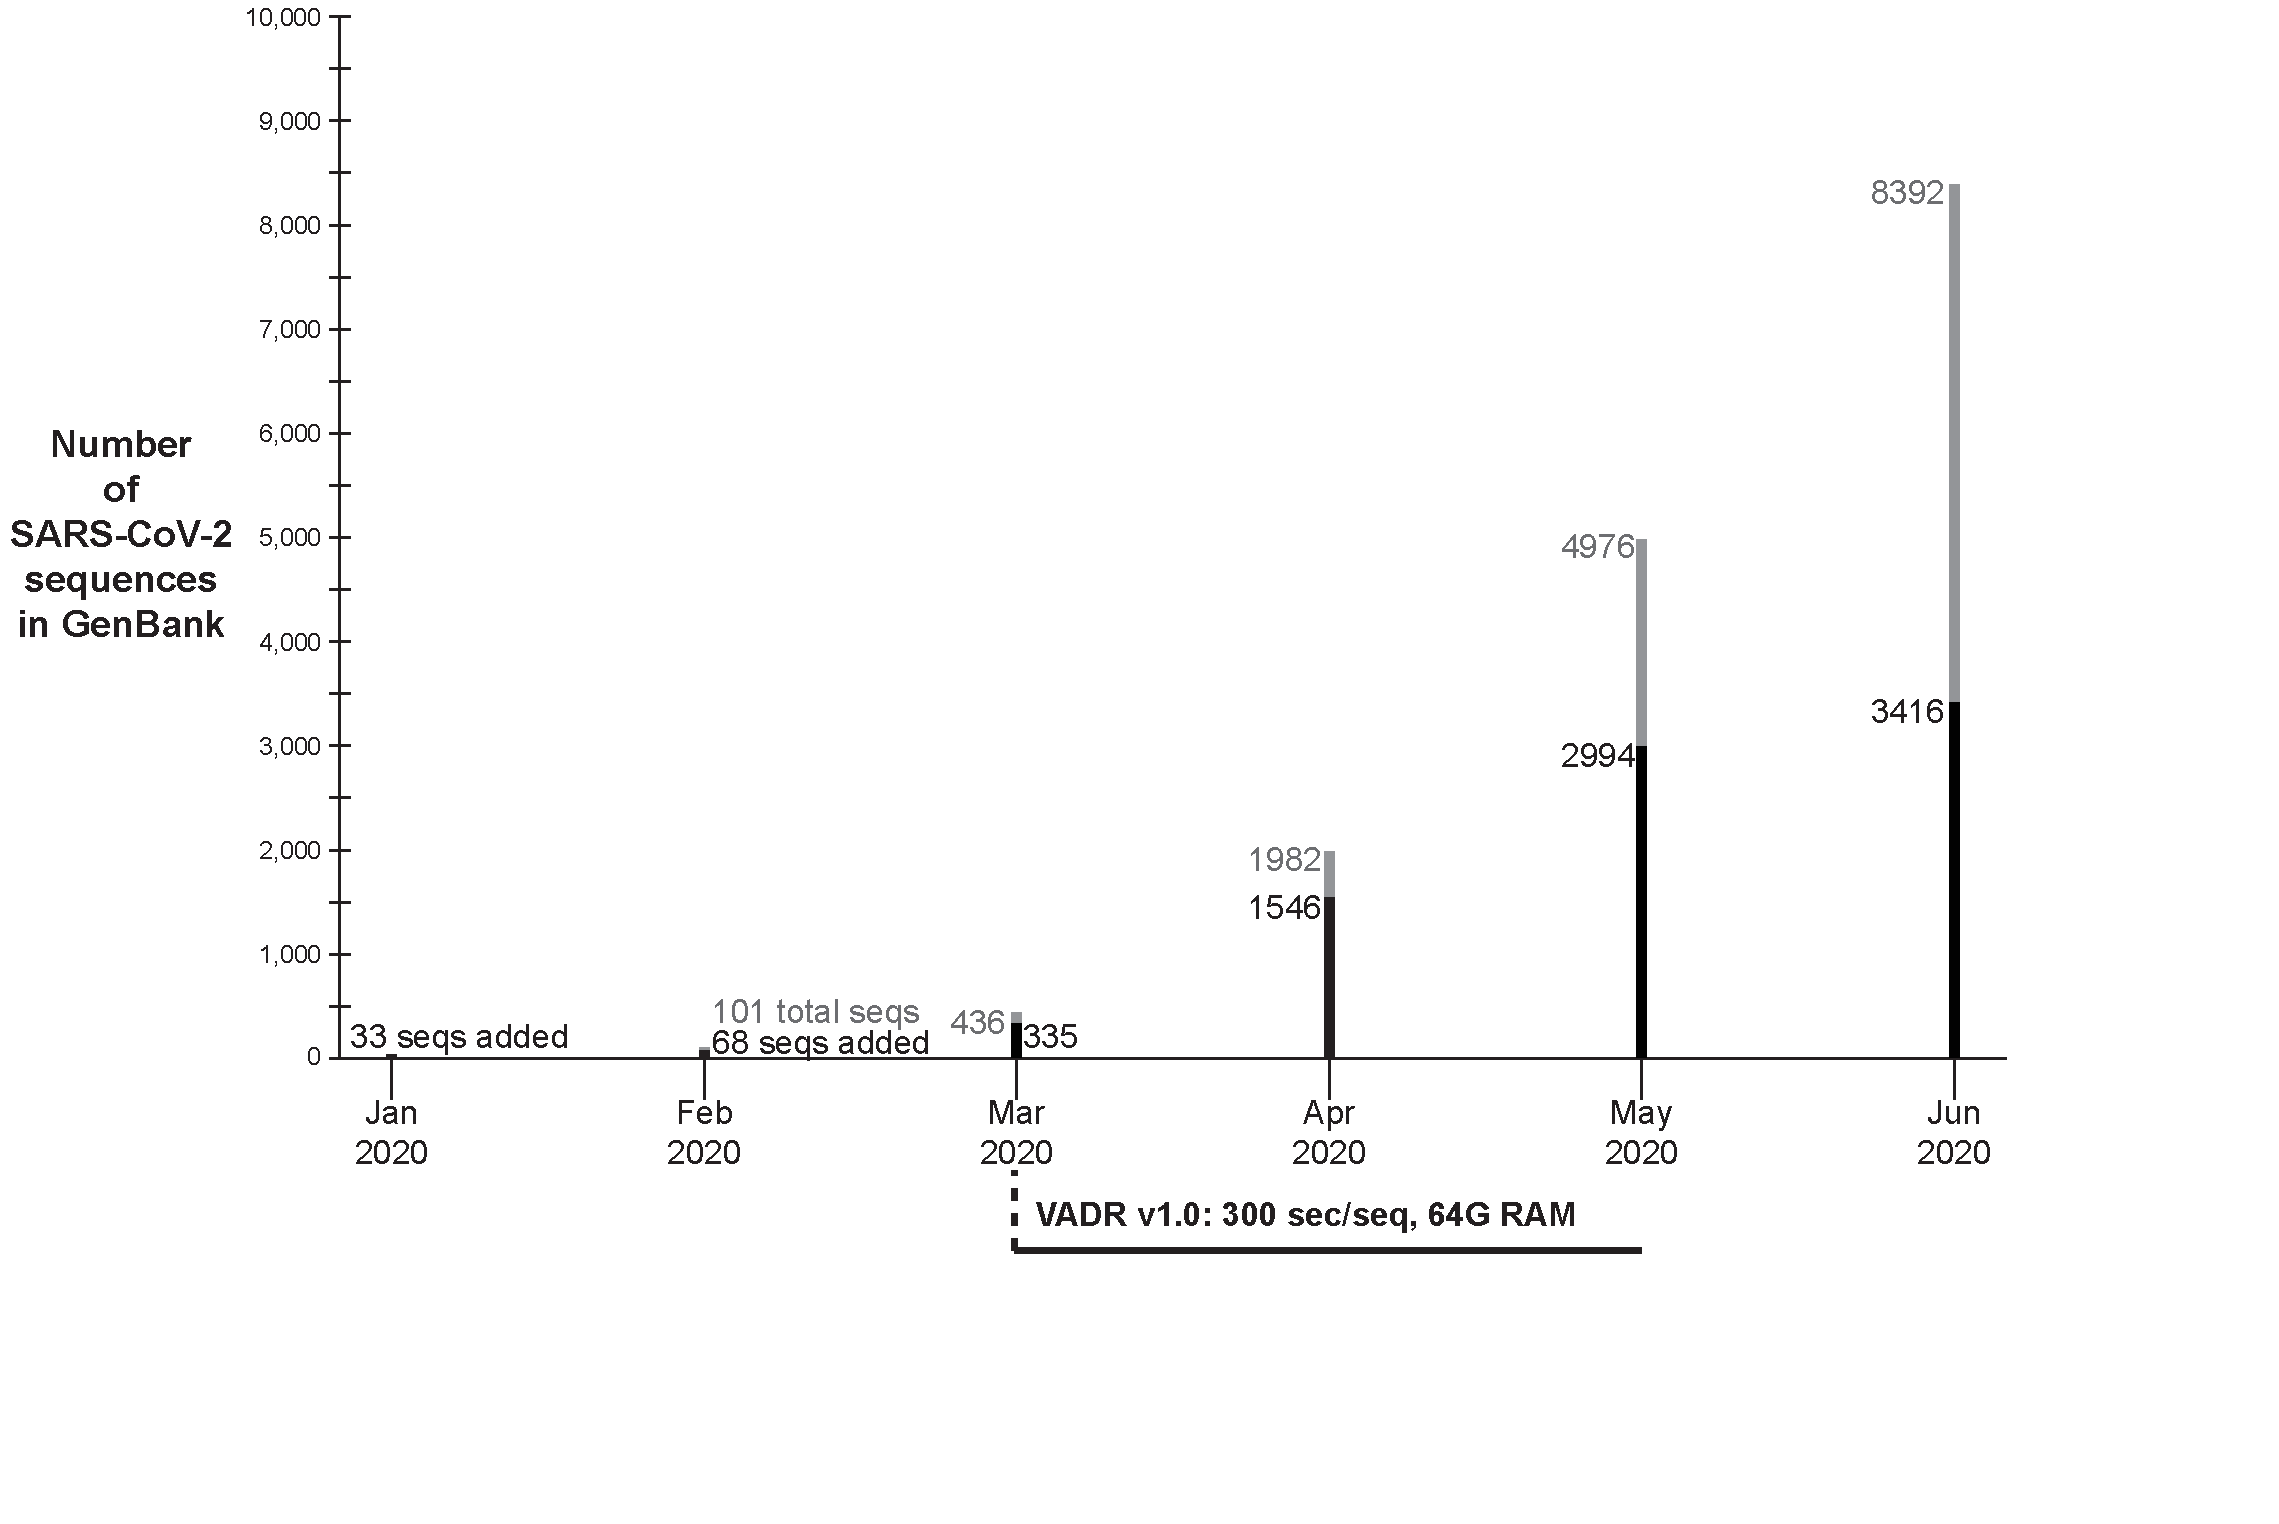
\includegraphics[width=10.5in]{figs/sars-counts-jan2020-may2020-slide2}
\end{center}

\vfill
\end{slide}
%%%%%%%%%%%%%%%%%%%%%%%%%%%%%%%%%%%%%%%%%%%%%%%%%%%%%%%%%%%%%%%%%%%%%%
\begin{slide}
\begin{center}
\textbf{SARS-CoV-2 sequences are N-rich}
\end{center}

\begin{center}
\begin{tabular}{lrr}
            & \% of nucleotides & \% of seqs w/stretch \\
  virus     & that are Ns       & of Ns $>=$ 50 nt     \\ \hline
& & \\
Dengue virus  & 0.0037\%        & 0.0070\%             \\
& & \\                    
Norovirus     & 0.296\%         & 0.628\%             \\
& & \\                    
SARS-CoV-2    & 1.12\%          & \emph{26.4\%}       \\
\end{tabular}
\end{center}
\vfill

\vfill
\end{slide}
%%%%%%%%%%%%%%%%%%%%%%%%%%%%%%%%%%%%%%%%%%%%%%%%%%%%%%%%%%%%%%%%%%%%%%
\begin{slide}
\begin{center}
\textbf{SARS-CoV-2 sequences are N-rich}
\end{center}

\begin{center}
\begin{tabular}{lrr}
            & \% of nucleotides & \% of seqs w/stretch \\
  virus     & that are Ns       & of Ns $>=$ 50 nt     \\ \hline
& & \\
Dengue virus  & 0.0037\%        & 0.0070\%             \\
& & \\                    
Norovirus     & 0.296\%         & 0.628\%             \\
& & \\                    
SARS-CoV-2    & 1.12\%          & \emph{26.4\%}       \\
\end{tabular}
\end{center}
\vfill

\begin{itemize}
\item
  N-rich sequences fail VADR because all stages
  (especially coverage determination and protein validation) rely on global
  similarity in the input sequence.
\item
  VADR 1.1 identifies stretches of Ns and replaces them with the
  homologous RefSeq sequence, annotates them, then places Ns back in.
\end{itemize}

\vfill
\end{slide}
%%%%%%%%%%%%%%%%%%%%%%%%%%%%%%%%%%%%%%%%%%%%%%%%%%%%%%%%%%%%%%%%%%%%%%
\begin{slide}
\begin{center}
\textbf{SARS-CoV-2 sequences (especially early ones) are all highly
  similar to the reference (typically $>$ 99.5\%)}
\end{center}

\begin{itemize}
\item VADR 1.1 exploits this high similarity by using faster methods
  \begin{itemize}
  \item blastn replaces cmsearch in classification and coverage determination stages
  \item Max ungapped blastn alignment region \emph{seeds} the cmalign alignment
  \end{itemize}
\end{itemize}

\vfill
\end{slide}
%%%%%%%%%%%%%%%%%%%%%%%%%%%%%%%%%%%%%%%%%%%%%%%%%%%%%%%%%%%%%%%%%%%%%%
\begin{slide}
\begin{center}
\textbf{VADR 1.1: 150X speedup on typical sequences}

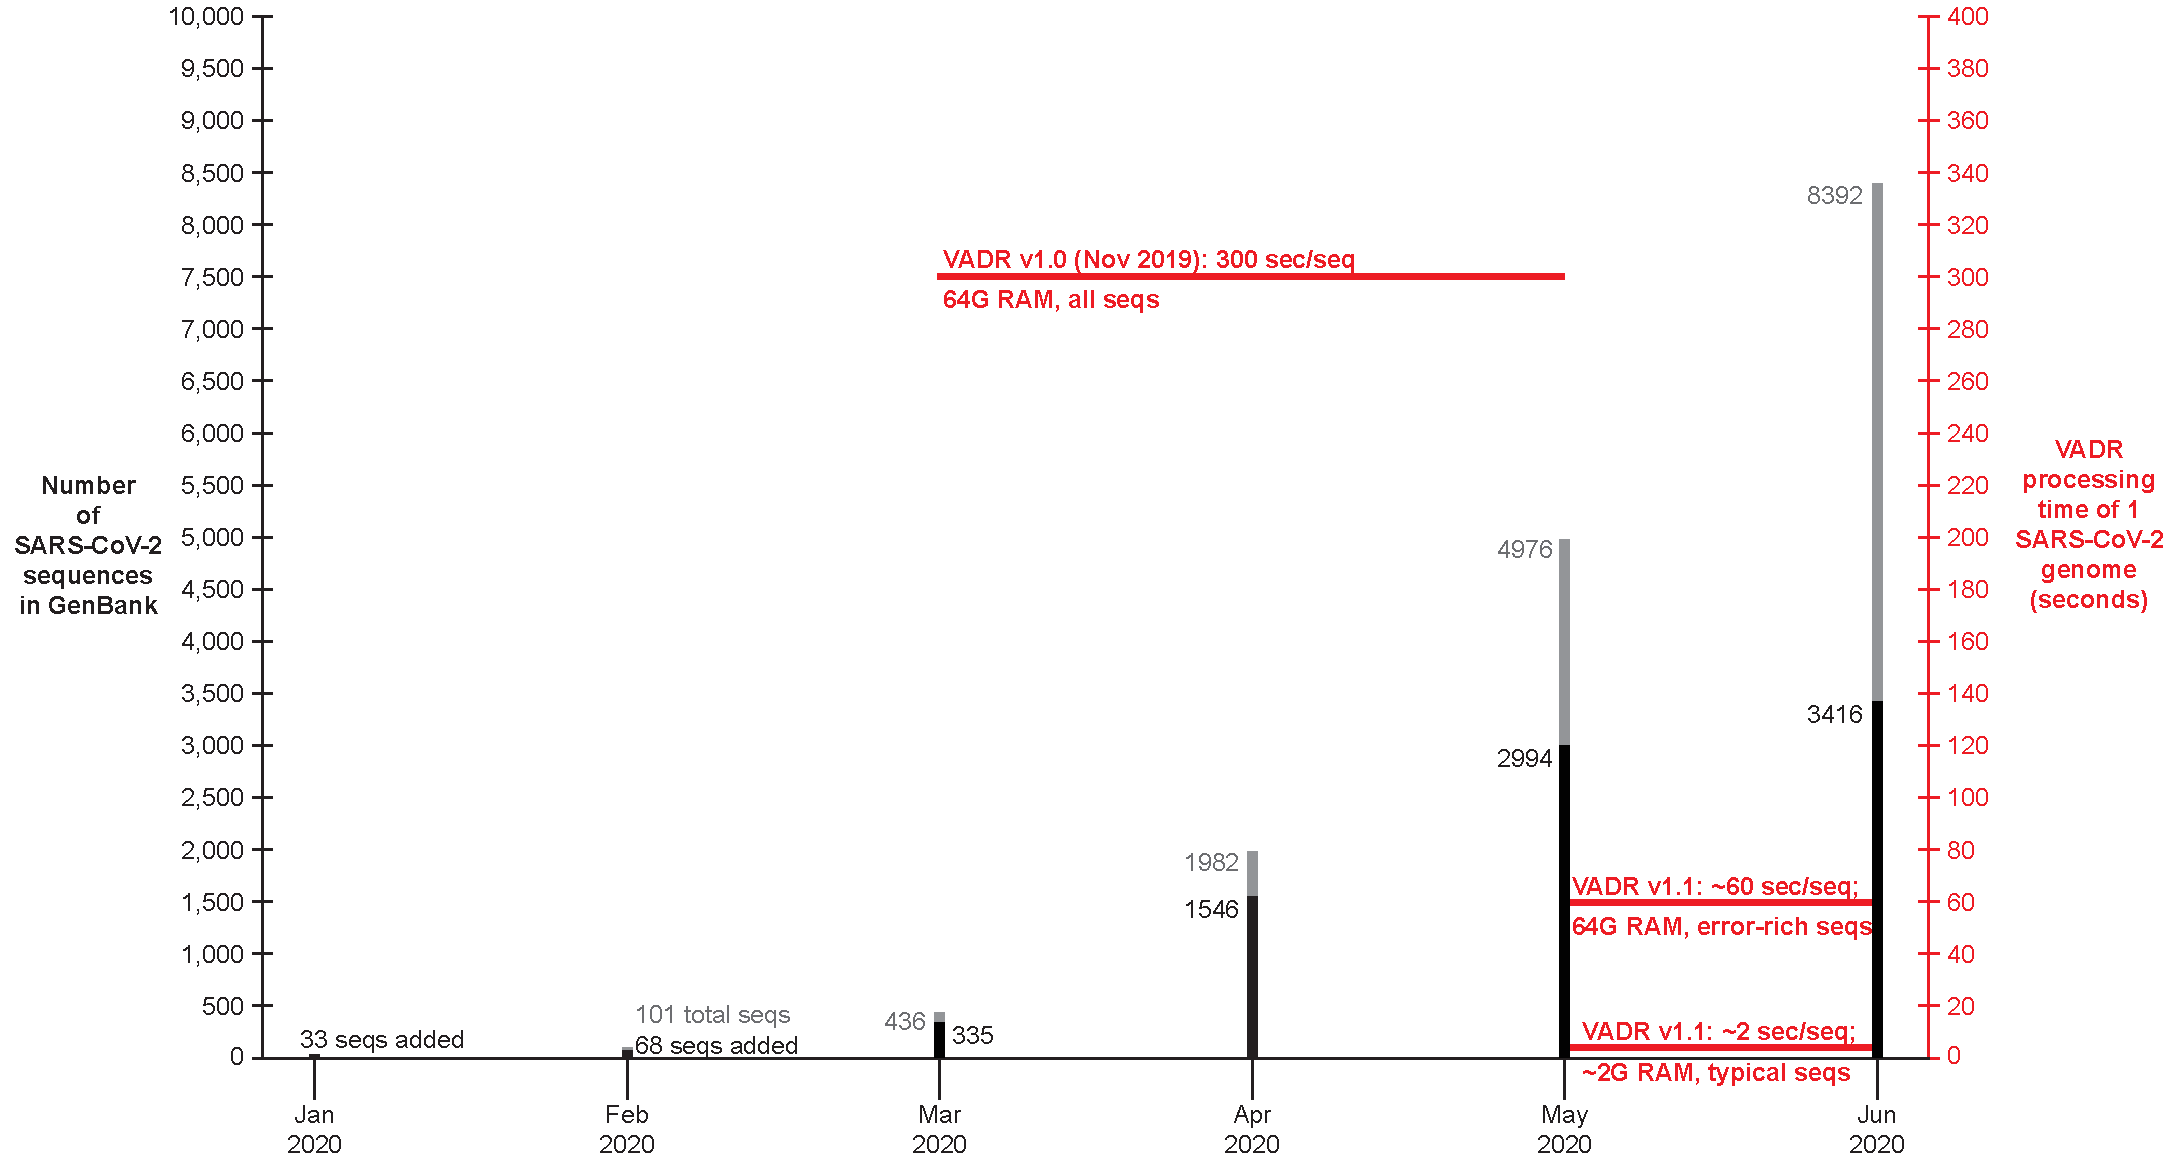
\includegraphics[width=10.5in]{figs/sars-counts-jan2020-may2020-slide3}
\end{center}

\vfill
\end{slide}
%%%%%%%%%%%%%%%%%%%%%%%%%%%%%%%%%%%%%%%%%%%%%%%%%%%%%%%%%%%%%%%%%%%%%%
\begin{slide}
\begin{center}
\Large{\textbf{Sequence volume increase in 2021}}

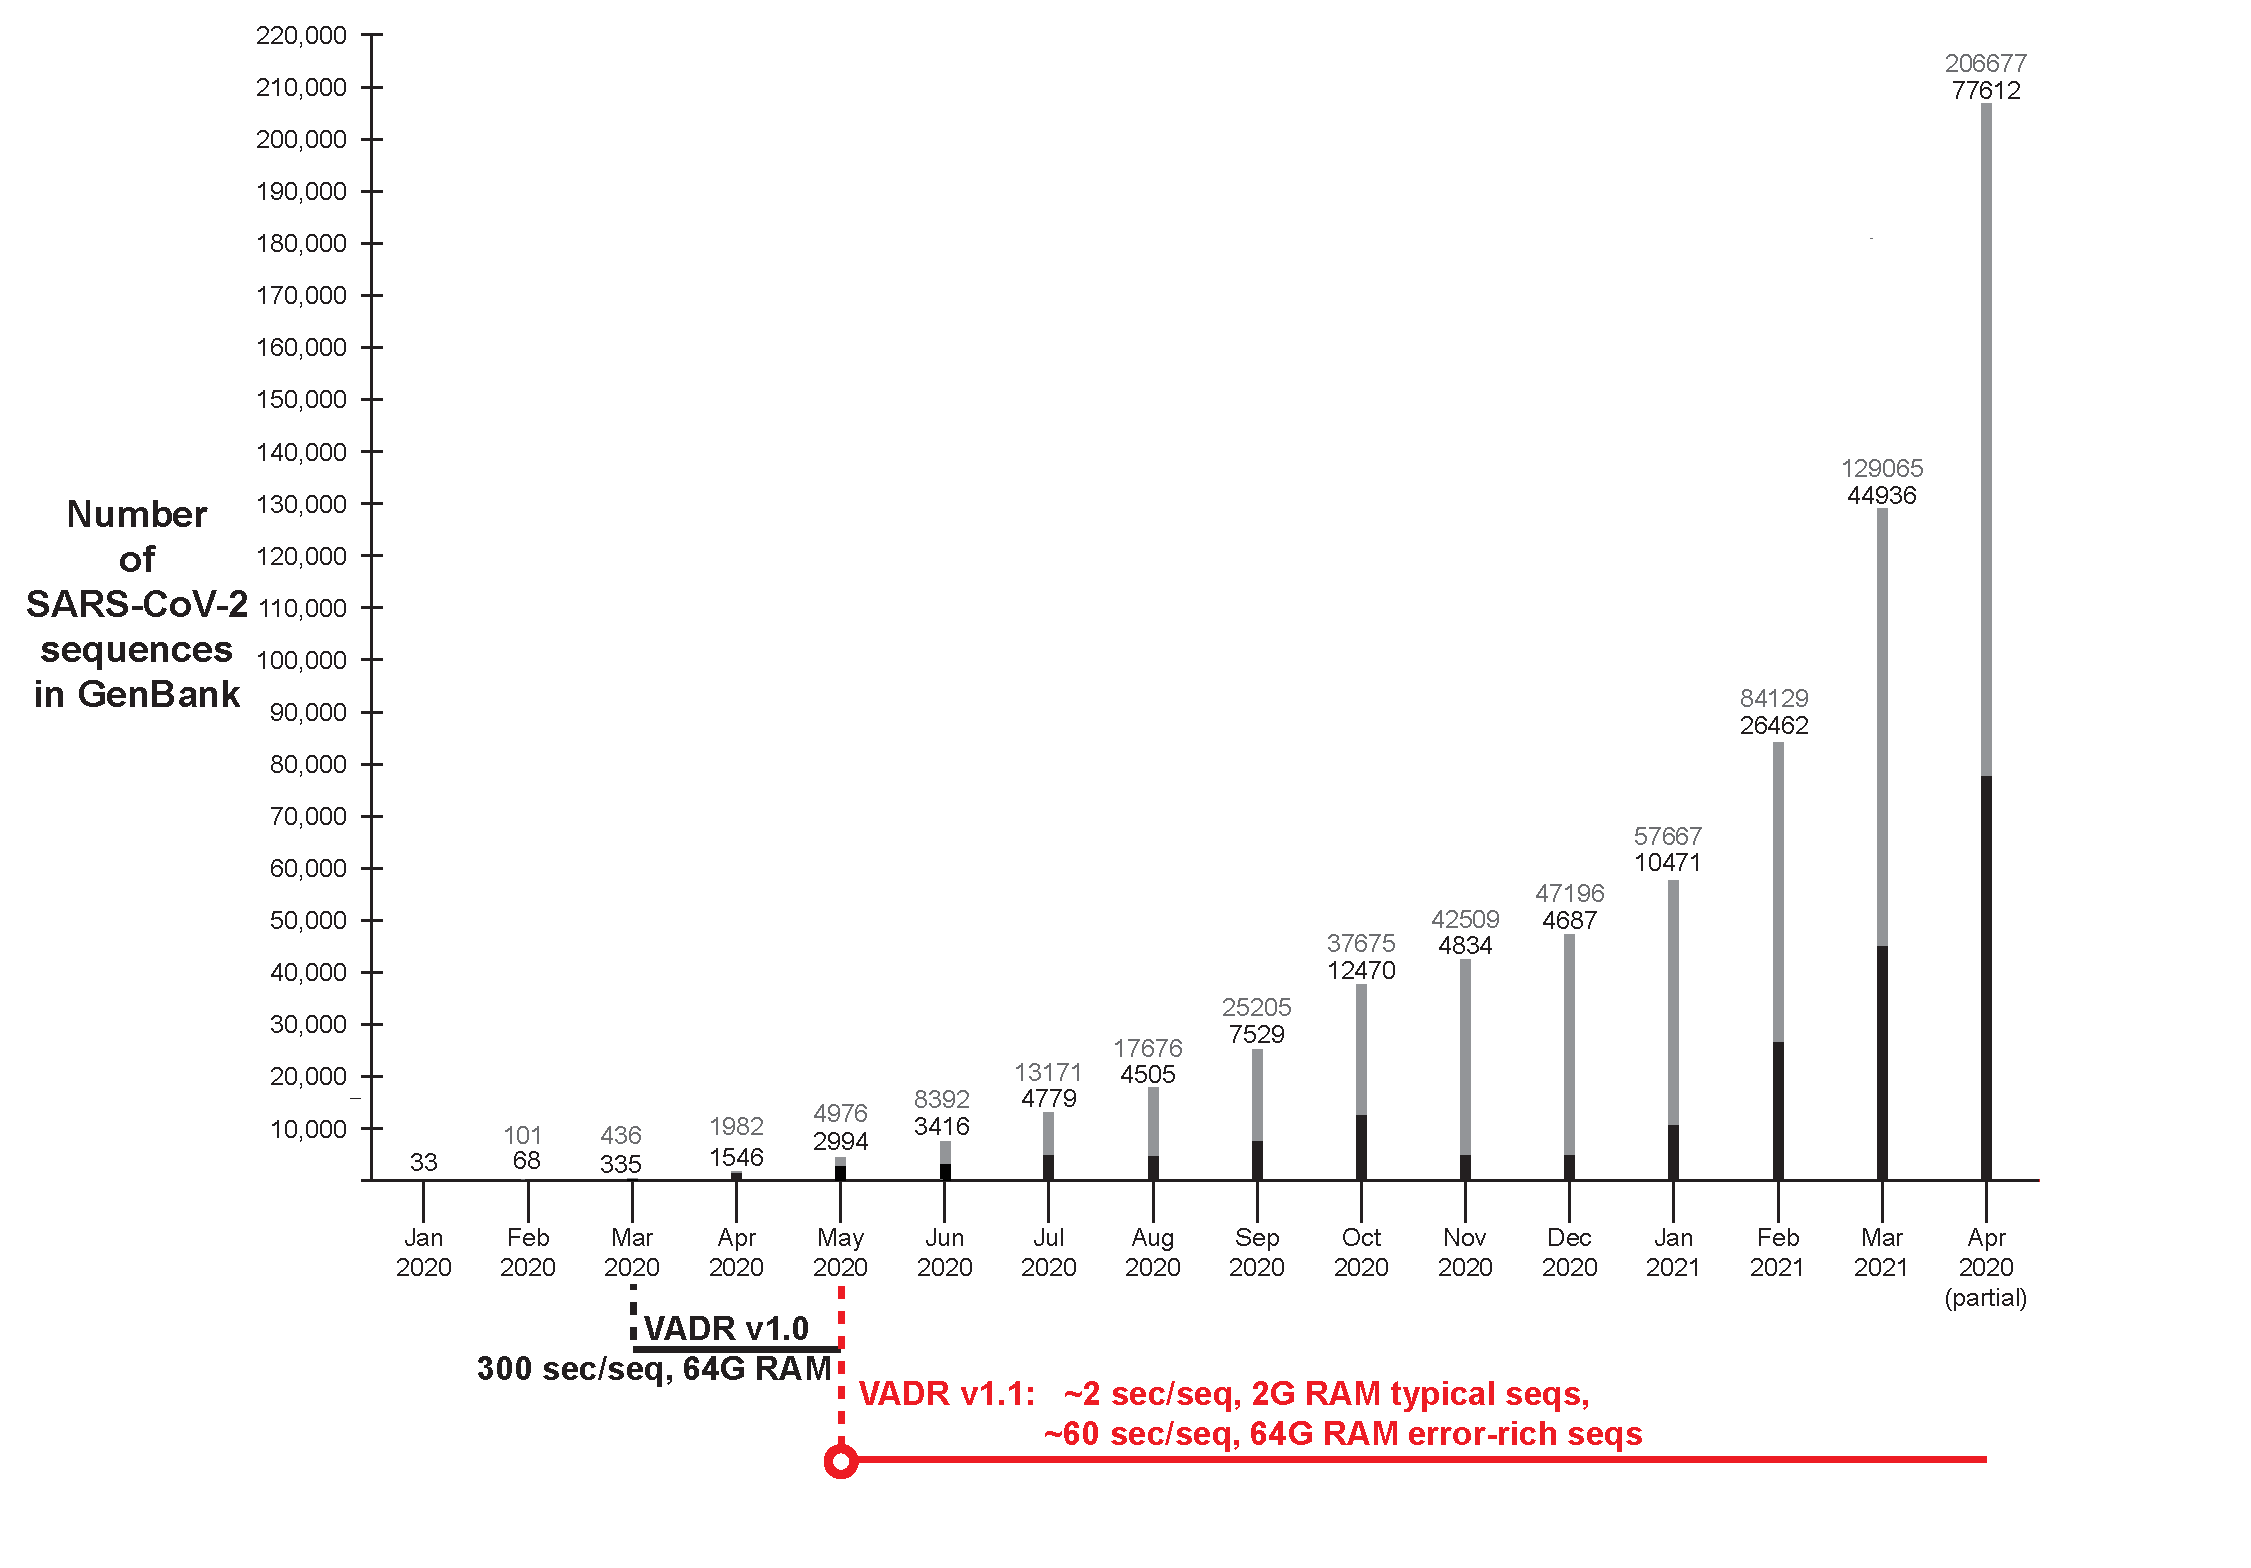
\includegraphics[width=10.5in]{figs/sars-counts-jan2020-apr2021-slide1}
\end{center}

\vfill
\end{slide}
%%%%%%%%%%%%%%%%%%%%%%%%%%%%%%%%%%%%%%%%%%%%%%%%%%%%%%%%%%%%%%%%%%%%%%
\begin{slide}
\begin{center}
\textbf{The glsearch program in the FASTA package does glocal
  alignment quicker and in less memory than cmalign}
\end{center}

\begin{itemize}
\item VADR 1.2 replaces cmalign with glsearch
  \begin{itemize}
  \item lower memory requirement opens door for multi-threading
  \item input file is split into chunks
    \begin{itemize}
    \item each chunk processed independently in parallel on one of 8 CPUs
    \item further reduces memory requirement (dependent on chunk size
      instead of full input file size)
    \end{itemize}
  \end{itemize}
\end{itemize}
  
\vfill
\end{slide}
%%%%%%%%%%%%%%%%%%%%%%%%%%%%%%%%%%%%%%%%%%%%%%%%%%%%%%%%%%%%%%%%%%%%%%
\begin{slide}
\begin{center}
\Large{\textbf{VADR v1.2 is 5-10X faster than v1.1}}

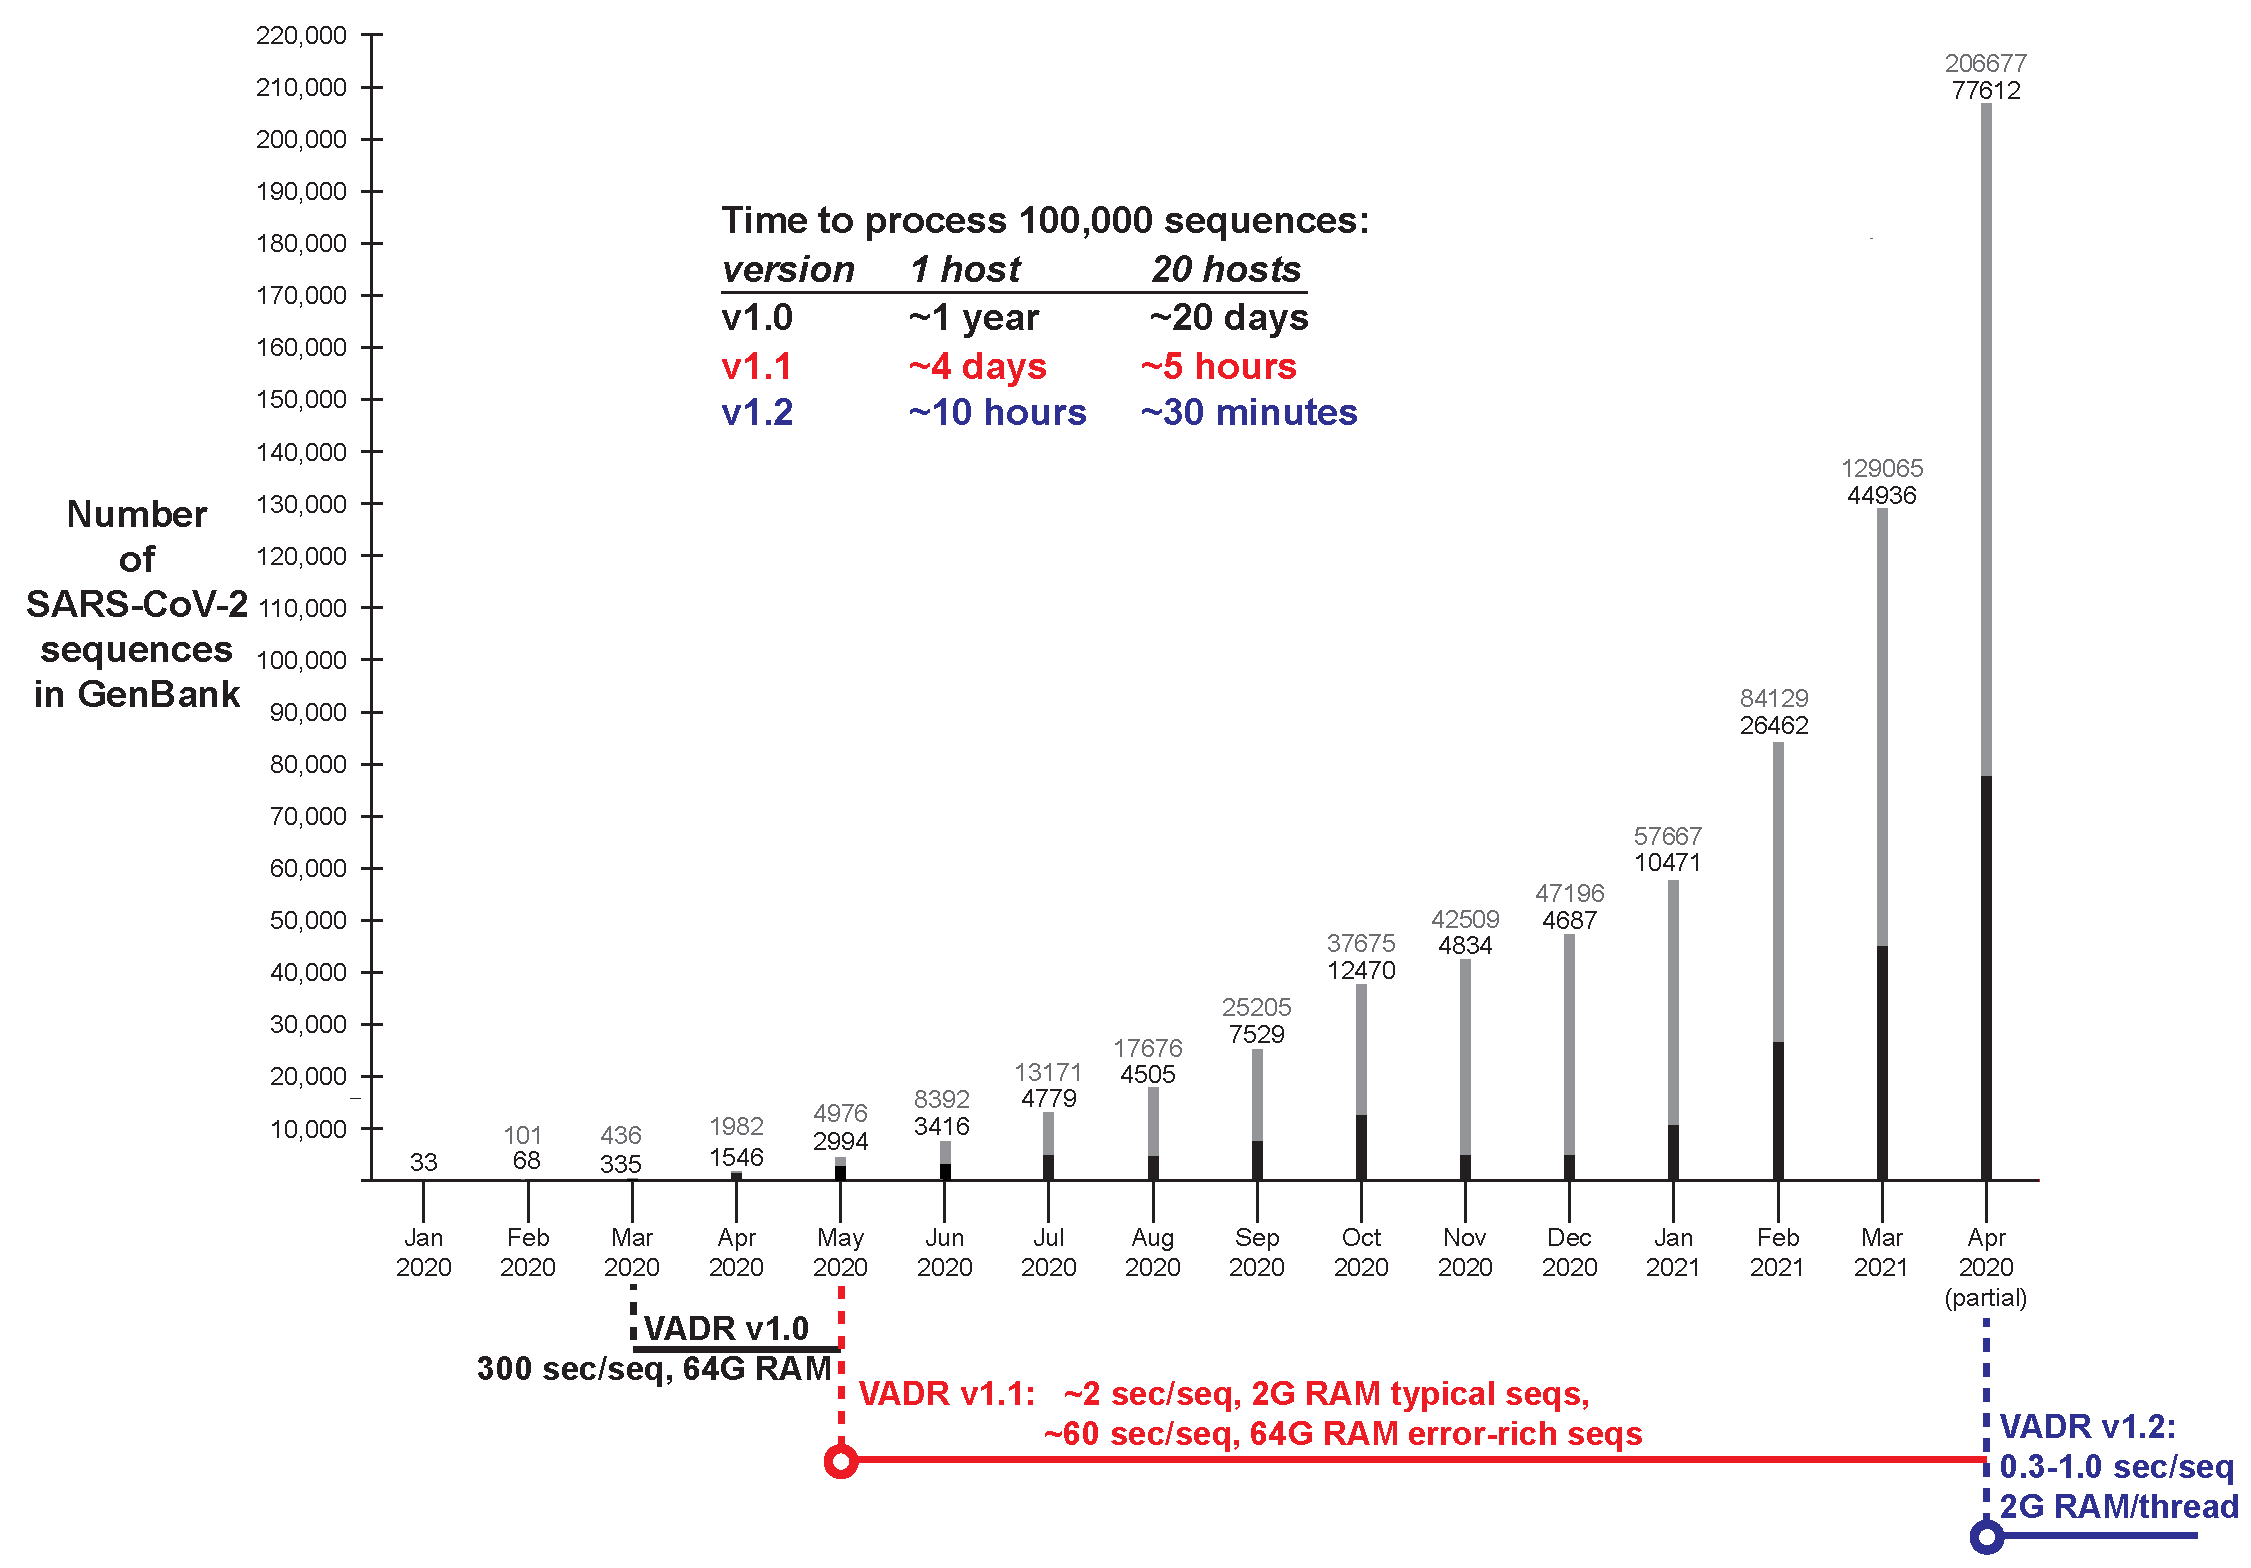
\includegraphics[width=10.5in]{figs/sars-counts-jan2020-apr2021-slide2}
\end{center}

\vfill
\end{slide}
%%%%%%%%%%%%%%%%%%%%%%%%%%%%%%%%%%%%%%%%%%%%%%%%%%%%%%%%%%%%%%%%%%%%%%
\begin{slide}
\begin{center}
\Large{\textbf{GenBank is now better prepared for upcoming onslaught of sequence submissions}}

\includegraphics[width=10.5in]{figs/sars-counts-jan2020-apr2021-slide3}
\end{center}

\vfill
\end{slide}
%%%%%%%%%%%%%%%%%%%%%%%%%%%%%%%%%%%%%%%%%%%%%%%%%%%%%%%%%%%%%%%%%%%%%%
\begin{slide}
\begin{center}
\Large{\textbf{Besides getting faster, VADR has improved in other ways}}

\begin{itemize}
\item Jan  8, 2021: B.1.1.7 model
\item Feb 12, 2021: VADR 1.1.3: more flexible to allow errors in ORF8 (or any
  specified CDS) 
\item Apr 12, 2021: B.1.525 model (49nt deletion that removes a stem loop)
\end{itemize}
\end{center}

\vfill
\end{slide}
%%%%%%%%%%%%%%%%%%%%%%%%%%%%%%%%%%%%%%%%%%%%%%%%%%%%%%%%%%%%%%%%%%%%%%
\begin{slide}
\begin{center}
\Large{\textbf{We verify VADR passes new SARS-CoV-2 lineages}}

\begin{itemize}
\item screenshot or latex table showing 43 variants COV-226 and that
  they all pass vadr (lineage name, mutlist, pass/fail)
\end{itemize}
\end{center}

\vfill
\end{slide}
%%%%%%%%%%%%%%%%%%%%%%%%%%%%%%%%%%%%%%%%%%%%%%%%%%%%%%%%%%%%%%%%%%%%%%
\begin{slide}
\begin{center}
\Large{\textbf{We actively support (and are supported by) the SPHERES community}}

\includegraphics[width=8in]{figs/spheres-slack-apr132021}

\begin{itemize}
\item VADR is portable and is run locally by labs prior to submission
\item docker container thanks to Curtis Kapsak and StaPH-B
\item SPHERES members alert us of problems with VADR and model coverage
\item We have weekly calls with CDC and receive questions and feature requests
\end{itemize}

\end{center}

\vfill
\end{slide}
%%%%%%%%%%%%%%%%%%%%%%%%%%%%%%%%%%%%%%%%%%%%%%%%%%%%%%%%%%%%%%%%%%%%%%
\begin{slide}
\begin{center}
\Large{\textbf{Future improvements: VADR 1.2.1 TODO list}}

\begin{itemize}
\item Review list of seqs that fail VADR but should pass
\item Review VADR error messages, and add parseable position data (SPHERES)
\item Handling of non NNN start/stop codons that translate to X (CDC)
\end{itemize}

\end{center}

\vfill
\end{slide}
%%%%%%%%%%%%%%%%%%%%%%%%%%%%%%%%%%%%%%%%%%%%%%%%%%%%%%%%%%%%%%%%%%%%%%
\begin{slide}

\large
\begin{center}
\large{\textbf{Acknowledgements}} \\

\normalsize
\vspace{0.75in}

\small
\begin{tabular}{l|l|l}
%                  & \\ \hline
%                  & \\
\textbf{NCBI - viral annotation} & \textbf{NCBI - leadership} &  \textbf{Other} \\
Alejandro Sch\"{a}ffer (now NCI) & David Landsman             & Sean Eddy (HMMER/Infernal/Easel)\\
Rodney Brister                   & Kim Pruitt                 & Travis Wheeler (HMMER)\\
Ilene Mizrachi                   & Jim Ostell                 & Tom Madden, Stephen Altschul, others (BLAST)\\
Colleen Bollin                   & David Lipman               & William Pearson (FASTA/glsearch) \\
Eneida Hatcher                   &                            & Michael Farrar (HMMER/glsearch) \\
Linda Yankie                     &                            & \\
Vincent Calhoun                  & \textbf{NLM - leadership}  & \\
Beverly Underwood                & Patti Brennan              & \\
Vasuki Gobu                      & Jerry Sheehan              &  \\
Sergiy Gotvyanskyy               &                            & \\
Alex Kotliarov                   &                            & \\
Lara Shonkwiler                  & & \\
Sophia Hu                        & & \\
\end{tabular}

\includegraphics[width=2.5in]{figs/NIH_NLM_ABRV_2C_4-white}
\includegraphics[width=2.5in]{figs/ncbi-logo}

\end{center}

\vfill
\end{slide}
%%%%%%%%%%%%%%%%%%%%%%%%%%%%%%%%%%%%%%%%%%%%%%%%%%%%%%%%%%%%%%%%%%%%%%
\end{document}
